\section{Implementierung}\label{kapitel6}
%Code erklären, Cooler Shit, Jackson, Token, Spring Sec, srtm download?, Validierung, Logger
\subsection{Webserver}
\subsubsection{Controller}
Spring MVC ermöglicht das verteilen der Anfragen an sogenannte Controller.

Diese stellen im MVC-Muster die Schicht zwischen dem Modell, sprich den Daten, und dem View, also der Ausgabe der Informationen dar.

Die Klasse des Controllers muss mit @Controller oder @RestController annotiert sein.

Über den Controller lassen sich Anfragetyp und URL u.A. anhand der Annotation ``@RequestMapping'' angeben. Ansonsten ist dies mit Spring MVC stattdessen auch mittels XML möglich.

Zusätzlich können unterschiedliche HTTP-Statuscodes zurückgegeben werden. Diese werden mit der Klasse ResponseEntity umgesetzt.

Die Annotation @RequestBody bedeutet dass es sich bei dem Parameter um den Inhalt des Anfragekörpers handelt. Dieser wird mithilfe von Jackson deserialisiert. Mehr darüber befindet sich im Abschnitt~\ref{jackson}.

Als Beispiel dient hier die Methode POST auf die URL /group, also zum Anlegen einer Gruppe:
\lstset{language=java}
\begin{lstlisting}[frame=htrbl, caption={Controller zum Erstellen einer Gruppe}, breaklines=true]
@RequestMapping(value = "group", method = RequestMethod.POST)
    public ResponseEntity<GroupDAO> create(@RequestBody @Valid CreateGroupRequest request) {
        try {
            return new ResponseEntity<GroupDAO>(Groups.createGroup(request), HttpStatus.CREATED);
        } catch(UserNotFoundException e) {
            return new ResponseEntity<GroupDAO>(HttpStatus.BAD_REQUEST);
        } catch (Exception e) {
            logger.error(e);
            return new ResponseEntity<>(HttpStatus.INTERNAL_SERVER_ERROR);
        }
   }
\end{lstlisting}
\subsubsection{Sicherheit}
Der Webserver ist mit dem Framework Spring Security abgesichert. Die Authentifizierung war dabei kein Hauptaugenmerk der Arbeit, jedoch ist sie in Grundzügen umgesetzt worden. 

So ist der Server nur allgemein abgesichert. Hat der Nutzer ein gültiges Token hat er kompletten Zugriff auf die REST-API. Das ist natürlich keine Option für ein produktives System, das seine Nutzerdaten stärker absichern muss.

Der folgende Code befindet sich in der ApplicationContext.xml und sorgt dafür, dass sämtliche Anfragen bis auf die zum Anmelden und Registrieren von Nutzern authentifiziert sein müssen.
\lstset{language=xml}
\begin{lstlisting}[frame=htrbl, caption={Ausschnitt aus der Datei ApplicationContext.xml}, breaklines=true]
<security:http realm="Protected API" use-expressions="true" auto-config="false" create-session="stateless" entry-point-ref="CustomAuthenticationEntryPoint" authentication-manager-ref="authenticationManager">
        <security:custom-filter ref="authenticationTokenProcessingFilter" position="FORM_LOGIN_FILTER" />
        <security:intercept-url pattern="/login" access="permitAll"/>
        <security:intercept-url pattern="/user" method="POST" access="permitAll"/>
        <security:intercept-url pattern="/**" access="isAuthenticated()" />
</security:http>
\end{lstlisting}
\paragraph{Anmeldung}
Um sich zu anzumelden schickt der Nutzer eine Anfrage an den Server, die eine JSON mit den Attributen ``name'' und ``password'' an den Server. Stimmen diese mit den auf einem Nutzer auf der Datenbank überein antwortet der Server mit einem Token, welches der Nutzer für drei Tage nutzen kann um die authentifizierten Bereiche der API benutzen zu können. 
\begin{figure}[htb]
\centering
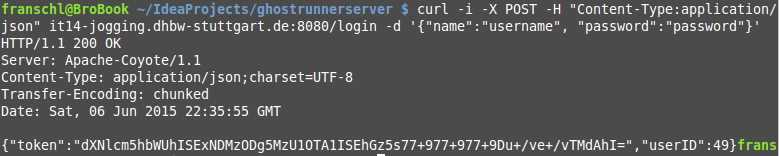
\includegraphics[width=\textwidth]{abb/curl_login}
\caption[Anmeldung]{Eine erfolgreiche Anmeldung mithilfe des Kommandozeilentools CURL}
\label{fig:Anmeldung}
\end{figure}
\paragraph{Authentifizierungstoken}
Das Authentifizierungstoken besteht, base64-dekodiert aus drei Teilen, getrennt durch jeweils drei Ausrufezeichen:
\begin{itemize}
\item Nutzername
\item Ablaufdatum des Tokens als UNIX-Zeitstempel (in Millisekunden)
\item geheimer Hash, der sich aus MD5-Hash des Nutzernamen, Salts und des Tokenablaufdatums zusammensetzt.
\end{itemize}

Dekodiert man z.B.  das erhaltene Token aus Abbildung~\ref{fig:Anmeldung} erhält man den folgenden String:
\begin{lstlisting}
username!!!1433889355905!!<eine Kette aus Sonderzeichen>
\end{lstlisting}
\paragraph{Nutzung des Sicherheitstokens}
Um sich mit dem Authentifizierungstoken am Server zu authentifizieren muss dieses bei jeder Anfrage des Klienten an den Server mitgeschickt werden.

Besonders zu Testzwecken empfiehlt es sich das Token per GET-Parameter in der URL mitzugeben. 

Eine Anfrage sieht dann z.B. so aus:
\begin{lstlisting}
it14-jogging.dhbw-stuttgart.de:8080/user/?token=<BeispielToken>
\end{lstlisting}

Eine weitere Option ist das Angeben des Tokens in der Kopzeile der Anfrage als das Attribut  ``authentication-token''.
\subsubsection{JSON - Serialisierung und Deserialisierung}\label{jackson}
Das Format der meisten Nachrichten zwischen Client und Server ist JSON.

Um den Aufwand zu minimieren und die Codeübersichtlichkeit zu maximieren wird dazu serverseitig das Tool Jackson in der Version 2.5.0 verwendet.

Es ist selbstständig in der Lage Klassen zu JSON-Objekten und Listen zu JSON-Arrays zu serialisieren und umgekehrt zu deserialisieren.

Die Einbindung erfolgt über Mavens pom.xml:
\lstset{language=xml}
\begin{lstlisting}[frame=htrbl, caption={Ausschnitt aus pom.xml}, breaklines=true]
<dependency>
	<groupId>com.fasterxml.jackson.core</groupId>
	<artifactId>jackson-core</artifactId>
	<version>2.5.0</version>
</dependency>

<dependency>
	<groupId>com.fasterxml.jackson.core</groupId>
	<artifactId>jackson-databind</artifactId>
	<version>2.5.0</version>
</dependency>

<dependency>
	<groupId>com.fasterxml.jackson.core</groupId>
	<artifactId>jackson-annotations</artifactId>
	<version>2.5.0</version>
</dependency>
\end{lstlisting}

In der mvc-dispatcher-servlet.xml wird die Bean eingebunden:
\lstset{language=xml}
\begin{lstlisting}[frame=htrbl, caption={Ausschnitt aus mvc-dispatcher-servlet.xml}, breaklines=true]
<bean id="jsonMessageConverter" class="org.springframework.http.converter.json.MappingJackson2HttpMessageConverter">
</bean>
\end{lstlisting}

Da Spring dank der ``component-scan''-Funktionalität von Spring MVC so konfiguriert ist, die Verzeichnisse automatisch nach Beans zu durchsuchen und diese einzubinden ist an dieser Stelle keine weitere Arbeit mehr nötig und Jackson tut seine Arbeit.

Wegen Hibernate kam es jedoch zu teils größeren Problemen mit Jackson. Diese liesen sich mittels einer weiteren Maven-Abhängigkeit eines speziell an Hibernate angepassten Jackson-Plugins und geringfügiger Änderungen im mvc-dispatcher-servlet.xml jedoch lösen:
\lstset{language=xml}
\begin{lstlisting}[frame=htrbl, caption={Ausschnitt aus der pom.xml}, breaklines=true]
<dependency>
	<groupId>com.fasterxml.jackson.datatype</groupId>
	<artifactId>jackson-datatype-hibernate4</artifactId>
	<version>2.4.0</version>
</dependency>
\end{lstlisting}
\lstset{language=xml}
\begin{lstlisting}[frame=htrbl, caption={Ausschnitt aus mvc-dispatcher-servlet.xml}, breaklines=true]
<mvc:annotation-driven>
        <mvc:message-converters>
            <bean class="org.springframework.http.converter.json.MappingJackson2HttpMessageConverter">
                <property name="objectMapper">
                    <bean class="com.springapp.HibernateAwareObjectMapper"/>
                </property>
            </bean>
        </mvc:message-converters>
    </mvc:annotation-driven>
\end{lstlisting}